\section*{Results}

\subsection*{A controlled benchmark isolates seven applicability invariants}

SituationCatch-Bench v0.1 contains 4,200 generated English instances, with 600
instances in each of seven diagnostic categories: temporal state change,
omitted answer-critical premises, source conflict, proposed versus confirmed
events, local versus universal scope, observer-dependent knowledge and real
versus counterfactual worlds. Every item provides a question, shuffled claims,
query time, required state variables, a gold action and, where answerable, a
gold answer. The benchmark is intentionally transparent: each category is a
software-level test of one applicability invariant rather than a claim to
natural linguistic diversity.

\begin{figure}[t]
\centering
\begin{tikzpicture}[node distance=7mm and 7mm, every node/.style={font=\small}]
\node[draw,rounded corners,align=center,minimum width=23mm] (e) {Evidence and\\query};
\node[draw,rounded corners,align=center,right=of e,minimum width=25mm] (s) {Situation\\sensing};
\node[draw,rounded corners,align=center,right=of s,minimum width=25mm] (u) {State update\\and validation};
\node[draw,rounded corners,align=center,right=of u,minimum width=25mm] (p) {Response\\policy};
\node[draw,rounded corners,align=center,below=of p,minimum width=26mm] (o) {Answer / retrieve /\\clarify / abstain};
\draw[-{Latex}] (e)--(s); \draw[-{Latex}] (s)--(u); \draw[-{Latex}] (u)--(p); \draw[-{Latex}] (p)--(o);
\end{tikzpicture}
\caption{Evaluation decomposition. The present experiment supplies oracle
structured situation variables and evaluates state update and response policy.
End-to-end research must additionally measure natural-language situation sensing.}
\label{fig:framework}
\end{figure}

\subsection*{Oracle-state control satisfies the generated invariants}

SCQA was compared with lexical retrieval, recency-ranked retrieval and a
latest-mention rule. All methods received the same generated claims; SCQA alone
used the complete oracle situation state and transition semantics. SCQA obtained
100.0\% action-and-answer accuracy. Latest mention obtained 85.7\%, recency
ranking 71.4\% and lexical retrieval 70.0\% (Fig.~\ref{fig:accuracy}). These
numbers are deterministic consequences of the benchmark and implementation and
should be interpreted as regression-test coverage, not as estimates of model
performance in a population of natural questions.

The 85.7\% value is structurally induced: the categories are equally weighted
and the latest-mention control systematically fails the hidden-premise category,
so success on six categories yields $6/7=85.7\%$. The 14.3 percentage-point gap
is therefore not presented as an empirical effect size against a competitive
baseline.

\begin{figure}[t]
\centering
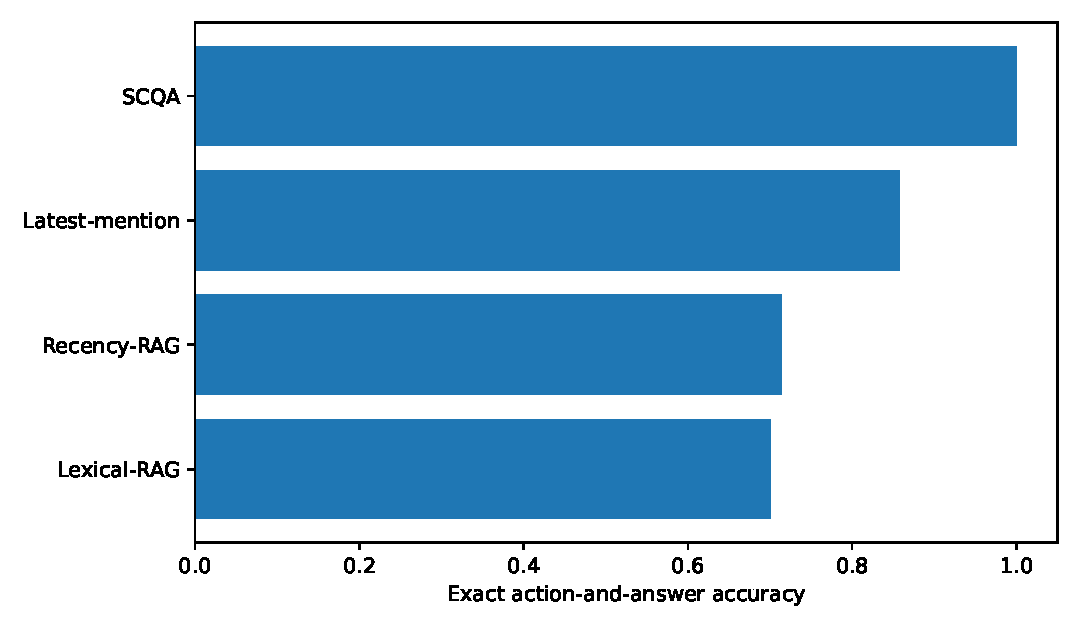
\includegraphics[width=.76\linewidth]{figures/accuracy.pdf}
\caption{Oracle-state diagnostic accuracy. The result demonstrates that the
specified invariants are executable. It does not estimate end-to-end LLM
accuracy because situation variables are supplied rather than inferred.}
\label{fig:accuracy}
\end{figure}

The category-level pattern provides the useful result. Latest mention fails on
hidden-premise items because it answers when clarification is required. Recency
ranking fails when the newest global event is not known to the queried observer.
Lexical overlap is vulnerable to weak but topically similar conflicting claims.
Thus a single aggregate ``hallucination'' label hides distinct and testable
mechanisms (Fig.~\ref{fig:category}).

\begin{figure}[t]
\centering
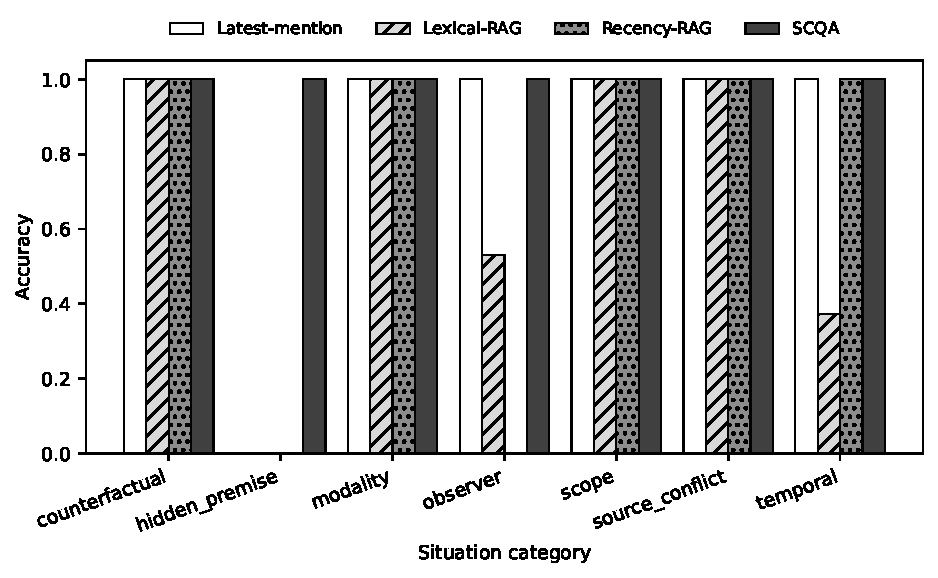
\includegraphics[width=.94\linewidth]{figures/by_category.pdf}
\caption{Accuracy by diagnostic category. Each category isolates one
applicability variable, enabling mechanism-level failure localization.}
\label{fig:category}
\end{figure}

\subsection*{Component ablations produce matched failure signatures}

Removing temporal validity, source status, modality, scope, observer knowledge,
world identity or missing-variable detection selectively damages the matching
category (Fig.~\ref{fig:ablation}). This causal alignment is the main empirical
contribution of the controlled study. It shows that the implementation does not
merely benefit from a generic instruction to be cautious; behaviour changes
when the specific variable required by an item is removed. Because benchmark
and solver share the same schema, the result is best viewed as a mechanistic
unit test that future neural systems should pass under both gold and predicted
states.

\begin{figure}[t]
\centering
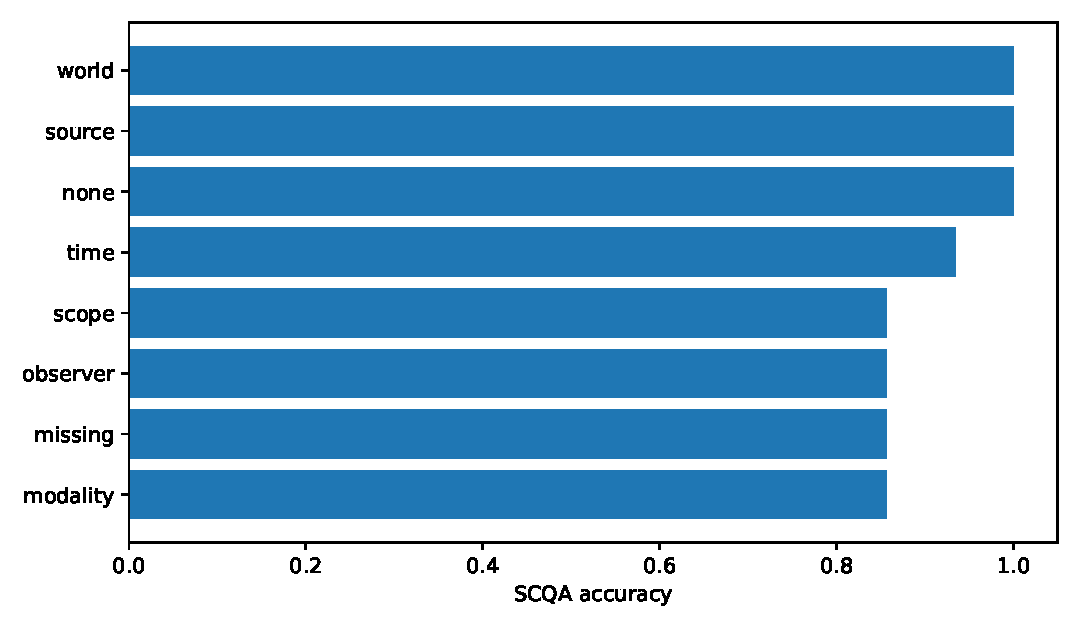
\includegraphics[width=.76\linewidth]{figures/ablations.pdf}
\caption{Oracle-state component ablations. Each removed variable recovers the
predicted category-specific failure, providing a causal software diagnostic.}
\label{fig:ablation}
\end{figure}

\subsection*{Predicted states expose a sensing bottleneck}

We removed access to the structured claim fields and reconstructed a restricted
situation state from claim text using the released deterministic sensor. Across
all 4,200 diagnostic instances, action-and-answer accuracy fell from 100.0\%
with gold states to 77.9\% with predicted states. Deliberately overwriting
source status, modality and scope in the predicted state reduced accuracy
further to 35.1\%. These are complete executions, not projected values. They
show that the oracle result is not preserved when situation sensing is
imperfect. Because the texts are generated from the same seven scenario
families and the sensor is a transparent rule baseline, these results remain
controlled diagnostics rather than evidence of natural-language or LLM
generalization.

Claim-level scoring localizes the sensor's limitations
(Table~\ref{tab:slot-sensing}). Event type reached 92.3\%, modality 100.0\%,
scope 61.5\%, actor 30.8\% and joint source/status 30.8\%. Temporal expressions
and validity intervals scored 0\% because the generated claim strings omit the
numeric times stored in the hidden schema: a system cannot reconstruct a state
variable that is neither expressed nor retrieved. Observer and world slots
reached 92.3\% and 100.0\% under repetitive generated language and are not
estimates of natural extraction. In this deterministic pipeline, 927 final
errors are attributable to sensing, zero to update/policy under gold state, and
generation is a fixed renderer.

\begin{table}[t]
\caption{Claim-level accuracy of the deterministic text sensor
($n=7{,}800$ claims per slot).}
\label{tab:slot-sensing}
\centering\scriptsize
\setlength{\tabcolsep}{3pt}%
\begin{tabular}{lrrrrrrrrr}
\toprule
Slot & Actor & Event & Time & Validity & Scope & Modality & Source & Observer & World\\
\midrule
Accuracy (\%) & 30.8 & 92.3 & 0.0 & 0.0 & 61.5 & 100.0 & 30.8 & 92.3 & 100.0\\
\bottomrule
\end{tabular}
\end{table}

\subsection*{Natural-language benchmarks establish prevalence, not SCQA efficacy}

Independent resources show that situation dependence is not confined to the
generated benchmark. SituatedQA reported that approximately 16.5\% of sampled
NQ-Open questions depended on time or place and that updated evidence did not
remove a substantial present-time performance gap~\cite{zhang2021situatedqa}.
FreshQA, PAT-Questions, TimeQA, ChronoQA and TDBench test related problems in
freshness, evolving facts and temporal validity
~\cite{vu2023freshqa,meem2024pat,chen2021timeqa,chen2025chronoqa,kim2025tdbench}.
These studies motivate the problem definition, but they are not evaluations of
SCQA and are not counted as evidence that the proposed intervention improves a
frontier model.

\subsection*{An evidence ladder separates established findings from open claims}

Table~\ref{tab:evidence-ladder} makes the claim boundary explicit. The current
study establishes that seven applicability invariants can be represented,
executed and independently ablated under oracle structured states. It supports,
but does not establish, the hypothesis that explicit situation states will
reduce analogous errors in LLMs. End-to-end efficacy requires matched
multi-model experiments on natural text, predicted-state evaluation, strong
prompt/RAG/agent baselines, clustered uncertainty estimates, human annotation
and efficiency analysis. We release the adapter, schemas and reporting protocol
for these experiments but do not substitute unexecuted predictions for results.

\begin{table}[t]
\caption{Evidence ladder and permitted interpretation.}
\label{tab:evidence-ladder}
\centering\small
\begin{tabularx}{\linewidth}{@{}>{\raggedright\arraybackslash}p{3.0cm}X>{\raggedright\arraybackslash}p{4.2cm}@{}}
\toprule
Evidence level & What is available & Permitted claim \\
\midrule
E1: formal definition & Situation schema and applicability relation & The failure class is operationally testable \\
E2: oracle unit tests & 4,200 generated instances and matched ablations & Specified invariants are executable and causally separable \\
E3: natural prevalence & Independent temporal/situated QA literature & Situation dependence occurs in natural questions \\
E4: predicted-state control & Deterministic text sensor on 4,200 generated items & Sensing errors reduce controlled end-to-end accuracy; natural-text generalization remains open \\
E5: multi-model intervention & Execution harness only; no successful model responses & Needed to claim LLM improvement and generality \\
E6: deployment / human study & Not completed & Needed for operational safety and human comparison \\
\bottomrule
\end{tabularx}
\end{table}
